\section{Circuitos integrados}

\frame{
	\frametitle{Introdução}
	\begin{block}{Definição}
		Os circuitos integrados são circuitos eletrônicos funcionais, constituídos por um conjunto de transistores, diodos, resistências e condensadores, fabricados num mesmo processo, sobre uma substância comum semicondutora de silício que se designa vulgarmente por chip.
	\end{block}

	\vspace{0.5cm}
	
	\centerline{\includegraphics[width=1\linewidth]{Figuras/Ch10/CI1.PNG}}
}

\frame{
	\frametitle{Vantagens e limitações}
	\begin{block}{Vantagens}
		\begin{itemize}
			\item Redução de custos, peso e tamanho.
			\item Maior velocidade de trabalho.
			\item Menor consumo de energia.
			\item Redução dos erros de montagem.
			\item Melhoria das características técnicas do circuito.
			\item Simplifica ao máximo a produção industrial.
		\end{itemize}
	\end{block}
}

\frame{
	\frametitle{Vantagens e limitações}
	\begin{block}{Limitações}
		\begin{itemize}
			\item Limitação nos valores das resistências e condensadores.
			\item Reduzida potência de dissipação.
			\item Limitações nas tensões de funcionamento.
			\item Impossibilidade de integrar num chip bobinas ou indutâncias.
		\end{itemize}
	\end{block}
}

\frame{
	\frametitle{Escala de integração e nanotecnologia}
	\begin{block}{}
		As portas não são vendidas individualmente, mas
		agrupadas em um circuito integrado (chip). Variam de acordo com seu tamanho:
		
		\begin{itemize}
			\item \textbf{SSI (Small Scale Integration)} - 1 a 12 portas.
			\item \textbf{MSI (Medium Scale Integration)} - 13 a 99 portas.
			\item \textbf{LSI (Large Scale Integration)} - 100 a \num{9999} portas.
			\item \textbf{VLSI (Very Large Scale Integration)} - \num{10000} a \num{99999} portas.
			\item \textbf{ULSI (Ultra Large Scale Integration)} - Acima de \num{100000} portas.
		\end{itemize}
	\end{block}
}

\frame{
	\frametitle{Como funciona?}
	\centerline{\includegraphics[height=0.9\textheight]{Figuras/Ch10/CI21.jpg}}
}

\frame{
	\frametitle{Como funciona?}
	\centerline{\includegraphics[height=0.9\textheight]{Figuras/Ch10/CI22.jpg}}
}

\frame{
	\frametitle{Como funciona?}
	\centerline{\includegraphics[height=0.9\textheight]{Figuras/Ch10/CI23.jpg}}
}

\frame{
	\frametitle{Como funciona?}
	\centerline{\includegraphics[width=0.8\linewidth]{Figuras/Ch10/CI3.jpg}}
}

\frame{
	\frametitle{Famílias: TTL x CMOS}
	\begin{block}{Introdução}
		\begin{itemize}
			\item Tipo de estrutura interna.
			\item Cada família utiliza determinados componentes em seus blocos.
			\item Diferentes características.
		\end{itemize}
	\end{block}
	\centerline{\includegraphics[width=0.5\linewidth]{Figuras/Ch10/TTLcmos.png}}
}

\frame{
	\frametitle{Conceitos - Níveis de tensão}
	\begin{block}{}
		\begin{itemize}
			\item Níveis $1$ e $0$ dentro de faixas.
		\end{itemize}
	\end{block}
	
	\centering
	\scalebox{0.8}{

\tikzset{every picture/.style={line width=0.75pt}} %set default line width to 0.75pt        

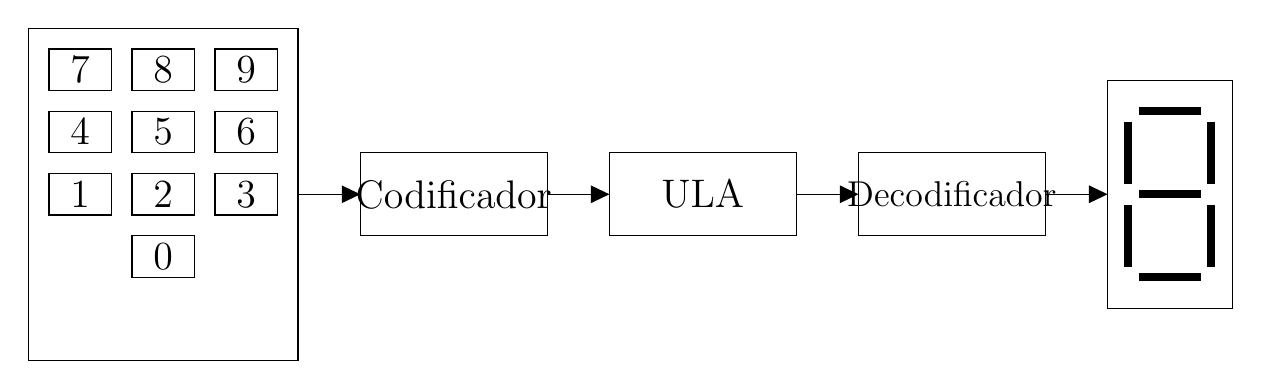
\begin{tikzpicture}[x=0.75pt,y=0.75pt,yscale=-1,xscale=1]
%uncomment if require: \path (0,300); %set diagram left start at 0, and has height of 300

%Shape: Rectangle [id:dp8798188650405219] 
\draw   (30,50) -- (160,50) -- (160,210) -- (30,210) -- cycle ;
%Shape: Rectangle [id:dp593444354888008] 
\draw   (40,60) -- (70,60) -- (70,80) -- (40,80) -- cycle ;
%Shape: Rectangle [id:dp4412846627526852] 
\draw   (80,60) -- (110,60) -- (110,80) -- (80,80) -- cycle ;
%Shape: Rectangle [id:dp2343273962035186] 
\draw   (120,60) -- (150,60) -- (150,80) -- (120,80) -- cycle ;
%Shape: Rectangle [id:dp05777918912875246] 
\draw   (40,90) -- (70,90) -- (70,110) -- (40,110) -- cycle ;
%Shape: Rectangle [id:dp9955010424516375] 
\draw   (80,90) -- (110,90) -- (110,110) -- (80,110) -- cycle ;
%Shape: Rectangle [id:dp24021539717259266] 
\draw   (120,90) -- (150,90) -- (150,110) -- (120,110) -- cycle ;
%Shape: Rectangle [id:dp36169684584711925] 
\draw   (40,120) -- (70,120) -- (70,140) -- (40,140) -- cycle ;
%Shape: Rectangle [id:dp7232437677097003] 
\draw   (80,120) -- (110,120) -- (110,140) -- (80,140) -- cycle ;
%Shape: Rectangle [id:dp6884539525496838] 
\draw   (120,120) -- (150,120) -- (150,140) -- (120,140) -- cycle ;
%Shape: Rectangle [id:dp9961423077173726] 
\draw   (80,150) -- (110,150) -- (110,170) -- (80,170) -- cycle ;
%Shape: Rectangle [id:dp6643057105712631] 
\draw   (190,110) -- (280,110) -- (280,150) -- (190,150) -- cycle ;
%Shape: Rectangle [id:dp7094011053258715] 
\draw   (550,75) -- (610,75) -- (610,185) -- (550,185) -- cycle ;
%Shape: Rectangle [id:dp2693438921699036] 
\draw   (310,110) -- (400,110) -- (400,150) -- (310,150) -- cycle ;
%Shape: Rectangle [id:dp3654960401722005] 
\draw   (430,110) -- (520,110) -- (520,150) -- (430,150) -- cycle ;
%Straight Lines [id:da6667328032348829] 
\draw    (160,130) -- (188,130) ;
\draw [shift={(190,130)}, rotate = 180] [fill={rgb, 255:red, 0; green, 0; blue, 0 }  ][line width=0.75]  [draw opacity=0] (8.93,-4.29) -- (0,0) -- (8.93,4.29) -- cycle    ;

%Straight Lines [id:da5165651690517046] 
\draw    (280,130) -- (308,130) ;
\draw [shift={(310,130)}, rotate = 180] [fill={rgb, 255:red, 0; green, 0; blue, 0 }  ][line width=0.75]  [draw opacity=0] (8.93,-4.29) -- (0,0) -- (8.93,4.29) -- cycle    ;

%Straight Lines [id:da17751850693095572] 
\draw    (400,130) -- (428,130) ;
\draw [shift={(430,130)}, rotate = 180] [fill={rgb, 255:red, 0; green, 0; blue, 0 }  ][line width=0.75]  [draw opacity=0] (8.93,-4.29) -- (0,0) -- (8.93,4.29) -- cycle    ;

%Straight Lines [id:da4998570413390182] 
\draw [color={rgb, 255:red, 0; green, 0; blue, 0 }  ,draw opacity=1 ][line width=3]    (560,95) -- (560,125) ;


%Straight Lines [id:da05287212083080073] 
\draw [color={rgb, 255:red, 0; green, 0; blue, 0 }  ,draw opacity=1 ][line width=3]    (600,95) -- (600,125) ;


%Straight Lines [id:da9146969001147236] 
\draw [color={rgb, 255:red, 0; green, 0; blue, 0 }  ,draw opacity=1 ][line width=3]    (560,135) -- (560,165) ;


%Straight Lines [id:da37610179690179124] 
\draw [color={rgb, 255:red, 0; green, 0; blue, 0 }  ,draw opacity=1 ][line width=3]    (600,135) -- (600,165) ;


%Straight Lines [id:da2798262228013664] 
\draw [color={rgb, 255:red, 0; green, 0; blue, 0 }  ,draw opacity=1 ][line width=3]    (595,130) -- (565,130) ;


%Straight Lines [id:da15184615547446478] 
\draw [color={rgb, 255:red, 0; green, 0; blue, 0 }  ,draw opacity=1 ][line width=3]    (595,90) -- (565,90) ;


%Straight Lines [id:da20609816632014244] 
\draw [color={rgb, 255:red, 0; green, 0; blue, 0 }  ,draw opacity=1 ][line width=3]    (595,170) -- (565,170) ;


%Straight Lines [id:da16937059284664002] 
\draw    (520,130) -- (548,130) ;
\draw [shift={(550,130)}, rotate = 180] [fill={rgb, 255:red, 0; green, 0; blue, 0 }  ][line width=0.75]  [draw opacity=0] (8.93,-4.29) -- (0,0) -- (8.93,4.29) -- cycle    ;


% Text Node
\draw (135,70) node   {\Large $9$};
% Text Node
\draw (95,70) node   {\Large $8$};
% Text Node
\draw (55,70) node   {\Large $7$};
% Text Node
\draw (135,100) node   {\Large $6$};
% Text Node
\draw (135,130) node   {\Large $3$};
% Text Node
\draw (95,160) node   {\Large $0$};
% Text Node
\draw (95,130) node   {\Large $2$};
% Text Node
\draw (95,100) node   {\Large $5$};
% Text Node
\draw (55,100) node   {\Large $4$};
% Text Node
\draw (55,130) node   {\Large $1$};
% Text Node
\draw (235,130) node  [align=left] {\Large Codificador};
% Text Node
\draw (355,130) node  [align=left] {\Large ULA};
% Text Node
\draw (475,130) node [scale=0.9] [align=left] {\Large Decodificador};


\end{tikzpicture}
}

%	\centerline{\includegraphics[width=0.7\linewidth]{Figuras/Ch10/tensao.png}}
}

\frame{
	\frametitle{Conceitos - Níveis de corrente}
	\begin{block}{De modo semelhante ao nível de tensão:}
		\begin{itemize}
			\item $I_{IL}$: valor de corrente máxima no terminal de entrada quando é aplicado nível 0
			\item $I_{OL}$: valor de corrente máxima que a saída pode receber quando em nível 0
			\item $I_{IH}$: valor de corrente máxima no terminal de entrada quando é aplicado nível 1
			\item $I_{OH}$: valor de corrente máxima que a saída pode receber quando em nível 1
		\end{itemize}
	\end{block}
}

\frame{
	\frametitle{Conceitos - \textit{Fan out}}
	\begin{block}{}
		\begin{itemize}
			\item A mesma saída pode ser usada para excitar diversas funções.
			\item A entrada de cada função precisa de certa corrente e a saída da função que vai excitar tem uma capacidade limitada de fornecimento de corrente.
		\end{itemize}
	\end{block}

	\begin{minipage}{0.45\textwidth}
		\begin{center}
			\centerline{\includegraphics[width=1\linewidth]{Figuras/Ch10/fanout1.png}}
		\end{center}
	
		\[ \text{\textit{fan-out} (Baixo)} = \dfrac{I_{OL\ (\text{max})}}{I_{IL\ (\text{max})}} \]
	\end{minipage}\hfill
	\begin{minipage}{0.45\textwidth}
		\begin{center}
			\centerline{\includegraphics[width=1\linewidth]{Figuras/Ch10/fanout2.png}}
		\end{center}
	
		\[ \text{\textit{fan-out} (Alto)} = \dfrac{I_{OH\ (\text{max})}}{I_{IH\ (\text{max})}} \]
	\end{minipage}
}

\frame{
	\frametitle{Conceitos - \textit{Fan in}}
	\begin{block}{}
		\begin{itemize}
			\item Definido como o número de entradas de determinada porta lógica
			\item Quanto maior este número, mais lenta será a porta.
		\end{itemize}
	\end{block}
	\centerline{\includegraphics[width=0.4\linewidth]{Figuras/Ch10/fanin.PNG}}
}

\frame{
	\frametitle{Conceitos - Tempo de atraso de propagação}
	\begin{block}{}
		\begin{itemize}
			\item Tempo que o bloco lógico leva para mudar de estado após uma mudança de nível.
			\item $t_{PLH}$: \textit{low} to \textit{high} - tempo para mudar de $0$ para $1$.
			\item $t_{PHL}$: \textit{high} to \textit{low} - tempo para mudar de $1$ para $0$.
		\end{itemize}
	\end{block}
	\centerline{\includegraphics[width=0.4\linewidth]{Figuras/Ch10/delay.png}}
}


\frame{
	\frametitle{A família TTL}
	\begin{block}{Conceitos}
		\begin{itemize}
			\item TTL significa Transistor-Transistor-Logic.
			\item A família TTL foi originalmente desenvolvida pela Texas Instruments.
			\item Série 74xx - comercial.
			\item Série 54xx - militar.
		\end{itemize}
	\end{block}
	\centerline{\includegraphics[width=0.4\linewidth]{Figuras/Ch10/CI5.jpg}}
}

\frame{
	\frametitle{A família TTL - Voltagem}
	\begin{block}{}
		\begin{itemize}
			\item Alimentado com uma tensão de \SI{5}{\volt}.
			\item Nível lógico $0$ é sempre a ausência de tensão ou \SI{0}{\volt}.
			\item Nível lógico $1$ é sempre uma tensão de \SI{5}{\volt}.
			\item Os níveis lógicos para serem reconhecidos devem estar dentro de faixas bem definidas. 
		\end{itemize}
	\end{block}
	\centerline{\includegraphics[width=0.6\linewidth]{Figuras/Ch10/ttltensao.png}}
}

\frame{
	\frametitle{A família TTL - Corrente}
	\begin{block}{}
		\begin{itemize}
			\item $I_{IL}$: \SI{1.6}{\milli\ampere}.
			\item $I_{OL}$: \SI{16}{\milli\ampere}.
			\item $I_{IH}$: \SI{40}{\micro\ampere}.
			\item $I_{OH}$: \SI{400}{\micro\ampere}.
		\end{itemize}
	\end{block}
}

\frame{
	\frametitle{A família TTL - Tempo de atraso}
	\begin{block}{}
		\begin{itemize}
			\item Valor médio de aproximadamente \SI{10}{\nano\second}, na versão \textit{standard}.
		\end{itemize}
	\end{block}
}


\frame{
	\frametitle{A família CMOS}
	\begin{block}{Conceitos}
		\begin{itemize}
			\item CMOS significa Complementary MOS.
			\item Transistores MOSFET.
			\item Série 4000A - comercial.
			\item Série 4000B - comercial.
			\item Série 54/74C - comercial - similar ao TTL.
			\item Série 74HC/74HCT - comercial - alta velocidade.
		\end{itemize}
	\end{block}

%	\vspace{0.3cm}
	\centerline{\includegraphics[width=0.4\linewidth]{Figuras/Ch10/CI4.png}}
}

\frame{
	\frametitle{A família CMOS - Voltagem}
	\begin{block}{}
		\begin{itemize}
			\item Série 4000/74C - $3$ a $\SI{15}{\volt}$
			\item Série 74HC - $2$ a $\SI{6}{\volt}$
			\item Série 74HCT - $\num{4.5}$ a $\SI{5.5}{\volt}$
		\end{itemize}
	\end{block}

	\medskip
	
	\centerline{\includegraphics[width=0.3\linewidth]{Figuras/Ch10/cmostensao.png}}
}

\frame{
	\frametitle{A família CMOS - Corrente}
	\begin{block}{}
		\begin{itemize}
			\item $I_{IL}$: \SI{1}{\micro\ampere}.
			\item $I_{OL}$: \SI{0.4}{\milli\ampere}.
			\item $I_{IH}$: \SI{1}{\micro\ampere}.
			\item $I_{OH}$: \SI{0.4}{\milli\ampere}.
		\end{itemize}
	\end{block}
}

\frame{
	\frametitle{A família CMOS - Tempo de atraso}
	\begin{block}{}
		\begin{itemize}
			\item Valor médio de aproximadamente \SI{90}{\nano\second}, nas séries mais comuns.
		\end{itemize}
	\end{block}
}

\frame{
	\frametitle{TTL x CMOS}
	\begin{block}{Comparação entre as famílias}
		\begin{itemize}
			\item A família CMOS possui maior imunidade a ruídos.
			\item A família CMOS possui um maior número de \textit{fan out}.
			\item Ao contrário da família TTL, na CMOS não é aconselhável deixar terminais de entradas desconectados. Estes devem ser ligados na tensão positiva ou terra, dependendo do modelo.
			\item A família CMOS trabalha com uma faixa maior para alimentação.
			\item A família TTL não possui problemas com o manuseio dos CI - eletricidade estática.
			\item A família TTL possui um tempo de atraso menor, se comparado com a CMOS.
		\end{itemize}
	\end{block}
}

\section*{Exercícios}

\frame{
	\frametitle{Exercícios}
	\begin{block}{}
		01. No último slide, têm-se a seguinte afirmação: \textit{``A família CMOS possui um maior número de fan out''.} Através dos conceitos e cálculos estudados, mostre que esta afirmação é verdadeira.
	\end{block}
}


\section*{Referências}

\frame{
	\frametitle{Referências e exercícios complementares}
	\begin{itemize}
		\item IDOETA, Ivan V. e CAPUANO, Francisco G. Elementos de Eletrônica Digital. São Paulo:
		      Editora Érica, ed. 40. 2008.
	\end{itemize}

	\centering{\alert{Página 469 - \textbf{9.8.9 até 9.8.11}}}

}